% Taller 4 -- Punto 3: Taller Propuesto de lógica difusa (revisión del script del profesor + desarrollo sobre Wine).  Compilar:  make punto3
% Las cifras (\cifra...) y las tablas salen de desarrollo/exportar_informe.py a partir de los cuadernos ejecutados.
\documentclass[11pt,letterpaper]{article}
\usepackage{ud-informe}
% Acento azul: el logo del programa (MCIC) es azul, así que se usa la gama azur del manual de marca en lugar del rojo.
% Para volver al rojo institucional de la plantilla, borrar estas dos líneas.
\colorlet{udrojo}{udazul}
\definecolor{udrojoosc}{HTML}{0C6F96}
% Generado por desarrollo/exportar_informe.py: NO editar a mano.
\newcommand{\cifrapropMamdani}{5,5586}
\newcommand{\cifrapropSugeno}{5,3445}
\newcommand{\cifrapropIrisReglas}{16}
\newcommand{\cifrapropIrisAcc}{0,889}
\newcommand{\cifrapropIrisAri}{0,729}
\newcommand{\cifratodoUnoA}{flavanoids}
\newcommand{\cifratodoUnoB}{proline}
\newcommand{\cifratodoUnoC}{OD280/OD315}
\newcommand{\cifratodoUnoD}{alcohol}
\newcommand{\cifratodoUnoFA}{188}
\newcommand{\cifratodoUnoFB}{149}
\newcommand{\cifratodoUnoFC}{127}
\newcommand{\cifratodoUnoFD}{100}
\newcommand{\cifrapropCurvaReglas}{0,2: 66, 0,3: 15, 0,4: 8, 0,5: 4, 0,6: 4, 0,7: 3, 0,8: 3, 0,9: 3, 1,0: 3}
\newcommand{\cifrapropRidgeSin}{45,1\,\%}
\newcommand{\cifrapropCvTresRidge}{90,3\,\%}
\newcommand{\cifrapropTestTresRidge}{96,3\,\%}
\newcommand{\cifrapropPureza}{0,927}
\newcommand{\cifrapropAri}{0,794}
\newcommand{\cifrapropFpc}{0,690}
\newcommand{\cifrapropFrontera}{20}
\newcommand{\cifrapropPurezaKm}{0,927}
\newcommand{\cifrapropMalAgrupados}{13}
\newcommand{\cifrapropRMejor}{0,8}
\newcommand{\cifrapropReglasMejor}{3}
\newcommand{\cifrapropAccMejor}{94,4\,\%}
\newcommand{\cifrapropCvUno}{45,1\,\%}
\newcommand{\cifrapropCvDos}{95,2\,\%}
\newcommand{\cifrapropCvTres}{96,0\,\%}
\newcommand{\cifratuneEntAntes}{0,145}
\newcommand{\cifratuneEntDesp}{0,095}
\newcommand{\cifratuneValAntes}{0,260}
\newcommand{\cifratuneValDesp}{0,254}
\newcommand{\cifratuneEntSin}{0,0006}
\newcommand{\cifratuneValSin}{0,384}
\newcommand{\cifratuneIter}{1}
\newcommand{\cifratuneIters}{40}
\newcommand{\cifratuneAccAntes}{90,7\,\%}
\newcommand{\cifratuneAccDesp}{94,4\,\%}
\newcommand{\cifratuneValSubida}{47}
\newcommand{\cifraveinteWMdos}{0,806 $\pm$ 0,049}
\newcommand{\cifraveinteReglasWMdos}{9,7 $\pm$ 1,2}
\newcommand{\cifraveinteWMtres}{0,865 $\pm$ 0,047}
\newcommand{\cifraveinteReglasWMtres}{24,1 $\pm$ 3,4}
\newcommand{\cifraveinteWMcuatro}{0,931 $\pm$ 0,036}
\newcommand{\cifraveinteReglasWMcuatro}{41,9 $\pm$ 2,9}
\newcommand{\cifraveinteSubTres}{0,881 $\pm$ 0,078}
\newcommand{\cifraveinteReglasSubTres}{14,8 $\pm$ 2,8}
\newcommand{\cifraveinteSubCinco}{0,956 $\pm$ 0,024}
\newcommand{\cifraveinteReglasSubCinco}{5,0 $\pm$ 0,9}
\newcommand{\cifraveinteSubOcho}{0,946 $\pm$ 0,024}
\newcommand{\cifraveinteReglasSubOcho}{3,0 $\pm$ 0,0}
\newcommand{\cifraveinteArbol}{0,894 $\pm$ 0,044}
\newcommand{\cifrapropSelDistintas}{2}
\newcommand{\cifrapropPermMax}{95,6\,\%}
\newcommand{\cifrapropPermMin}{90,4\,\%}
\newcommand{\cifrapropPermWM}{86,5\,\%}
\newcommand{\cifraadicN}{5456}
\newcommand{\cifraadicTrain}{3856}
\newcommand{\cifraadicTest}{1600}
\newcommand{\cifraadicDupCuatro}{50}
\newcommand{\cifraadicDupDos}{279}
\newcommand{\cifraadicRacha}{6,5}
\newcommand{\cifraadicCambios}{395}
\newcommand{\cifraadicSharp}{2097}
\newcommand{\cifraadicSlightR}{826}
\newcommand{\cifraadicForward}{2205}
\newcommand{\cifraadicSlightL}{328}
\newcommand{\cifraadicDosReglas}{6}
\newcommand{\cifraadicDosW}{0,02}
\newcommand{\cifraadicDosAcc}{99,81}
\newcommand{\cifraadicDosBal}{99,88}
\newcommand{\cifraadicDosF}{99,88}
\newcommand{\cifraadicDosMF}{2\,$\times$\,3}
\newcommand{\cifraadicCuatroReglas}{24}
\newcommand{\cifraadicCuatroW}{0,02}
\newcommand{\cifraadicCuatroAcc}{99,50}
\newcommand{\cifraadicCuatroBal}{99,39}
\newcommand{\cifraadicCuatroF}{99,45}
\newcommand{\cifraadicCuatroMF}{2\,$\times$\,3\,$\times$\,2\,$\times$\,2}
\newcommand{\cifraadicCorteFrente}{0,9005}
\newcommand{\cifraadicCorteIzqA}{0,4945}
\newcommand{\cifraadicCorteIzqB}{0,9015}
\newcommand{\cifraadicAutoDosMin}{91,4\,\%}
\newcommand{\cifraadicAutoDosMax}{96,1\,\%}
\newcommand{\cifraadicAutoCuatroMin}{78,7\,\%}
\newcommand{\cifraadicAutoCuatroMax}{95,2\,\%}
\newcommand{\cifraadicAutoReglasMin}{48}
\newcommand{\cifraadicAutoReglasMax}{100}
\newcommand{\cifraadicKnnBloques}{85,6\,\%}
\newcommand{\cifraadicKnnMuestra}{94,0\,\%}
\newcommand{\cifraadicKnnInfla}{8,3}
\newcommand{\cifraadicMamdaniDosCero}{97,8\,\%}
\newcommand{\cifraadicMamdaniDosGrande}{58,2\,\%}
\newcommand{\cifraadicGanadoraDosGrande}{92,6\,\%}


\renewcommand{\UDtitulo}{Taller propuesto de lógica difusa}
\renewcommand{\UDsubtitulo}{Revisión del script del profesor y desarrollo sobre el conjunto Wine}
\renewcommand{\UDtipo}{Taller 4 -- Punto 3 -- Informe de ejecución}
\renewcommand{\UDasignatura}{Inteligencia Computacional Aplicada}
\renewcommand{\UDdocente}{Cesar Andrey Perdomo Charry}
\renewcommand{\UDestudiantes}{Juan Felipe Rodríguez Galindo -- 20261595004}
\renewcommand{\UDencabezado}{Taller 4 -- Punto 3: taller propuesto}
\newcommand{\pts}{\,pts}

\begin{document}
\UDportada

%% ---------------------------------------------------------------------------------------------
\section{Revisión del script del profesor}

El script es el cuaderno \texttt{Taller\_LogicaDifusa\_RESUELTO\_Colab.ipynb} (Python, con su equivalente \texttt{Taller\_Resuelto\_profesor.mlx} en MATLAB). Recorre los bloques básicos de la lógica difusa:
funciones de pertenencia, operadores, un sistema Mamdani y uno Sugeno, un clasificador con reglas extraídas de los datos (Wang--Mendel simplificado) y Fuzzy C-Means (FCM), y los contrasta con \texttt{scikit-fuzzy}.
Para comprobar que cada bloque quedó entendido se reprodujeron con código propio sus valores de referencia (tabla~\ref{tab:ref}); los nueve coinciden.

La figura~\ref{fig:secuencia} muestra quién habla con quién. El \textbf{cuaderno} orquesta: pide grados de pertenencia, delega la inferencia en el motor (que repite el mismo ciclo por cada regla: fuzzificar, calcular la fuerza,
recortar la salida), compara con \texttt{scikit-fuzzy} y construye reglas a partir de datos.

\begin{figure}[H]
\centering
% Diagrama de secuencia (UML) del cuaderno resuelto de lógica difusa del profesor (Taller_LogicaDifusa_RESUELTO_Colab).
% Se incluye con % Diagrama de secuencia (UML) del cuaderno resuelto de lógica difusa del profesor (Taller_LogicaDifusa_RESUELTO_Colab).
% Se incluye con % Diagrama de secuencia (UML) del cuaderno resuelto de lógica difusa del profesor (Taller_LogicaDifusa_RESUELTO_Colab).
% Se incluye con \input{diagrama_secuencia_profesor} dentro de un entorno figure. Paleta de ud-informe.
\begin{tikzpicture}[yscale=0.76, font=\fontsize{7.6pt}{9pt}\selectfont,
    part/.style={draw=udsable!70, fill=white, rounded corners=2pt, minimum width=2.25cm, minimum height=0.7cm, align=center, inner sep=2pt},
    parthecho/.style={part, draw=udrojo, fill=udrojo!8, font=\fontsize{7.6pt}{9pt}\selectfont\bfseries},
    vida/.style={udplata!80, dash pattern=on 2.5pt off 2.5pt, line width=0.5pt},
    sync/.style={-{Latex[length=1.8mm]}, line width=0.65pt, color=udsable},
    retorno/.style={-{Latex[length=1.8mm, open]}, line width=0.55pt, color=udsable!65, dash pattern=on 3pt off 2pt},
    txt/.style={fill=white, inner sep=1.2pt, text=udsable},
    et/.style={txt, above=1.6pt},
    marco/.style={draw=udrojo!80, line width=0.7pt, rounded corners=1pt},
    etiq/.style={fill=udrojoosc, text=white, font=\fontsize{6.8pt}{8pt}\selectfont\bfseries, inner sep=2pt, anchor=north west},
    nota/.style={draw=udplata, fill=udfondo, font=\fontsize{7pt}{8.4pt}\selectfont, align=left, inner sep=3pt}]

  \def\xU{0.0}   \def\xC{2.95}  \def\xM{5.9}   \def\xI{8.85}  \def\xS{11.8}  \def\xR{14.75}
  \node[part]      at (\xU,0) {\textbf{Usuario}\\(estudiante)};
  \node[parthecho] at (\xC,0) {Cuaderno\\(Colab, Python)};
  \node[part]      at (\xM,0) {\texttt{MF y operadores}\\(\texttt{trimf}, \texttt{trapmf}, \ldots)};
  \node[part]      at (\xI,0) {Motor de\\inferencia};
  \node[part]      at (\xS,0) {\texttt{scikit-fuzzy}\\(referencia)};
  \node[part]      at (\xR,0) {Reglas desde datos\\(Wang--Mendel, FCM)};
  \foreach \x in {\xU,\xC,\xM,\xI,\xS,\xR} \draw[vida] (\x,-0.35) -- (\x,-18.3);

  % marco de repetición: una vuelta por cada regla del motor Mamdani
  \draw[marco] (\xM-0.5,-5.55) rectangle (\xI+0.6,-8.0);
  \node[etiq] at (\xM-0.5,-5.55) {loop \;\;para cada regla (3)};

  \draw[sync]    (\xU,-1.5)  -- node[et]{ejecutar pasos 0 a 7} (\xC,-1.5);
  \draw[sync]    (\xC,-2.2)  -- node[et]{\texttt{trimf(x, a, b, c)}} (\xM,-2.2);
  \draw[retorno] (\xM,-2.75) -- node[et]{grados $\mu\in[0,1]$} (\xC,-2.75);
  \draw[sync]    (\xC,-3.45) -- node[et]{\texttt{fuzz.trimf}: comparar} (\xS,-3.45);
  \draw[retorno] (\xS,-4.0)  -- node[et]{valores iguales} (\xC,-4.0);
  \draw[sync]    (\xC,-4.75) -- node[et]{\texttt{evaluar\_mamdani(servicio=1, comida=2)}} (\xI,-4.75);
  \draw[sync]    (\xI,-6.45) -- node[et]{$\mu$ de cada entrada} (\xM,-6.45);
  \draw[sync]    (\xI,-7.0)  -- (\xI+0.5,-7.0) -- (\xI+0.5,-7.45) -- (\xI,-7.45);
  \node[txt, anchor=west] at (\xI+0.6,-7.22) {fuerza (Y/O); recorte con mín};
  \draw[sync]    (\xI,-8.5)  -- (\xI+0.5,-8.5) -- (\xI+0.5,-8.95) -- (\xI,-8.95);
  \node[txt, anchor=west] at (\xI+0.6,-8.72) {agregación (máx) y centroide};
  \draw[retorno] (\xI,-9.6)  -- node[et]{propina = 5,5586} (\xC,-9.6);
  \draw[sync]    (\xC,-10.35)-- node[et]{\texttt{ControlSystemSimulation}} (\xS,-10.35);
  \draw[retorno] (\xS,-10.9) -- node[et]{5,5539 ($\approx$)} (\xC,-10.9);
  \draw[sync]    (\xC,-11.65)-- node[et]{\texttt{evaluar\_sugeno0}} (\xI,-11.65);
  \draw[retorno] (\xI,-12.2) -- node[et]{5,3445} (\xC,-12.2);
  \draw[sync]    (\xC,-13.0) -- node[et]{\texttt{extraer\_reglas(Iris, 3 MF)}} (\xR,-13.0);
  \draw[sync]    (\xR,-13.6) -- (\xR+0.5,-13.6) -- (\xR+0.5,-14.05) -- (\xR,-14.05);
  \node[txt, anchor=east] at (\xR-0.15,-13.82) {una regla por muestra; se queda la de mayor grado};
  \draw[retorno] (\xR,-14.7) -- node[et]{16 reglas} (\xC,-14.7);
  \draw[sync]    (\xC,-15.35)-- node[et]{\texttt{predecir\_reglas(prueba)}} (\xR,-15.35);
  \draw[retorno] (\xR,-15.9) -- node[et]{exactitud 0,889} (\xC,-15.9);
  \draw[sync]    (\xC,-16.6) -- node[et]{\texttt{fcm\_propio(c = 3)}} (\xR,-16.6);
  \draw[retorno] (\xR,-17.2) -- node[et]{ARI = 0,729} (\xC,-17.2);
  \draw[retorno] (\xC,-17.9) -- node[et]{\texttt{[OK]} / \texttt{[REVISAR]}} (\xU,-17.9);

  \node[nota, anchor=north east] at (\xR+0.55,-18.7) {Paso 7: repite \texttt{extraer\_reglas} con $n=2$ a 5 y compara con un árbol de decisión.};
\end{tikzpicture}
 dentro de un entorno figure. Paleta de ud-informe.
\begin{tikzpicture}[yscale=0.76, font=\fontsize{7.6pt}{9pt}\selectfont,
    part/.style={draw=udsable!70, fill=white, rounded corners=2pt, minimum width=2.25cm, minimum height=0.7cm, align=center, inner sep=2pt},
    parthecho/.style={part, draw=udrojo, fill=udrojo!8, font=\fontsize{7.6pt}{9pt}\selectfont\bfseries},
    vida/.style={udplata!80, dash pattern=on 2.5pt off 2.5pt, line width=0.5pt},
    sync/.style={-{Latex[length=1.8mm]}, line width=0.65pt, color=udsable},
    retorno/.style={-{Latex[length=1.8mm, open]}, line width=0.55pt, color=udsable!65, dash pattern=on 3pt off 2pt},
    txt/.style={fill=white, inner sep=1.2pt, text=udsable},
    et/.style={txt, above=1.6pt},
    marco/.style={draw=udrojo!80, line width=0.7pt, rounded corners=1pt},
    etiq/.style={fill=udrojoosc, text=white, font=\fontsize{6.8pt}{8pt}\selectfont\bfseries, inner sep=2pt, anchor=north west},
    nota/.style={draw=udplata, fill=udfondo, font=\fontsize{7pt}{8.4pt}\selectfont, align=left, inner sep=3pt}]

  \def\xU{0.0}   \def\xC{2.95}  \def\xM{5.9}   \def\xI{8.85}  \def\xS{11.8}  \def\xR{14.75}
  \node[part]      at (\xU,0) {\textbf{Usuario}\\(estudiante)};
  \node[parthecho] at (\xC,0) {Cuaderno\\(Colab, Python)};
  \node[part]      at (\xM,0) {\texttt{MF y operadores}\\(\texttt{trimf}, \texttt{trapmf}, \ldots)};
  \node[part]      at (\xI,0) {Motor de\\inferencia};
  \node[part]      at (\xS,0) {\texttt{scikit-fuzzy}\\(referencia)};
  \node[part]      at (\xR,0) {Reglas desde datos\\(Wang--Mendel, FCM)};
  \foreach \x in {\xU,\xC,\xM,\xI,\xS,\xR} \draw[vida] (\x,-0.35) -- (\x,-18.3);

  % marco de repetición: una vuelta por cada regla del motor Mamdani
  \draw[marco] (\xM-0.5,-5.55) rectangle (\xI+0.6,-8.0);
  \node[etiq] at (\xM-0.5,-5.55) {loop \;\;para cada regla (3)};

  \draw[sync]    (\xU,-1.5)  -- node[et]{ejecutar pasos 0 a 7} (\xC,-1.5);
  \draw[sync]    (\xC,-2.2)  -- node[et]{\texttt{trimf(x, a, b, c)}} (\xM,-2.2);
  \draw[retorno] (\xM,-2.75) -- node[et]{grados $\mu\in[0,1]$} (\xC,-2.75);
  \draw[sync]    (\xC,-3.45) -- node[et]{\texttt{fuzz.trimf}: comparar} (\xS,-3.45);
  \draw[retorno] (\xS,-4.0)  -- node[et]{valores iguales} (\xC,-4.0);
  \draw[sync]    (\xC,-4.75) -- node[et]{\texttt{evaluar\_mamdani(servicio=1, comida=2)}} (\xI,-4.75);
  \draw[sync]    (\xI,-6.45) -- node[et]{$\mu$ de cada entrada} (\xM,-6.45);
  \draw[sync]    (\xI,-7.0)  -- (\xI+0.5,-7.0) -- (\xI+0.5,-7.45) -- (\xI,-7.45);
  \node[txt, anchor=west] at (\xI+0.6,-7.22) {fuerza (Y/O); recorte con mín};
  \draw[sync]    (\xI,-8.5)  -- (\xI+0.5,-8.5) -- (\xI+0.5,-8.95) -- (\xI,-8.95);
  \node[txt, anchor=west] at (\xI+0.6,-8.72) {agregación (máx) y centroide};
  \draw[retorno] (\xI,-9.6)  -- node[et]{propina = 5,5586} (\xC,-9.6);
  \draw[sync]    (\xC,-10.35)-- node[et]{\texttt{ControlSystemSimulation}} (\xS,-10.35);
  \draw[retorno] (\xS,-10.9) -- node[et]{5,5539 ($\approx$)} (\xC,-10.9);
  \draw[sync]    (\xC,-11.65)-- node[et]{\texttt{evaluar\_sugeno0}} (\xI,-11.65);
  \draw[retorno] (\xI,-12.2) -- node[et]{5,3445} (\xC,-12.2);
  \draw[sync]    (\xC,-13.0) -- node[et]{\texttt{extraer\_reglas(Iris, 3 MF)}} (\xR,-13.0);
  \draw[sync]    (\xR,-13.6) -- (\xR+0.5,-13.6) -- (\xR+0.5,-14.05) -- (\xR,-14.05);
  \node[txt, anchor=east] at (\xR-0.15,-13.82) {una regla por muestra; se queda la de mayor grado};
  \draw[retorno] (\xR,-14.7) -- node[et]{16 reglas} (\xC,-14.7);
  \draw[sync]    (\xC,-15.35)-- node[et]{\texttt{predecir\_reglas(prueba)}} (\xR,-15.35);
  \draw[retorno] (\xR,-15.9) -- node[et]{exactitud 0,889} (\xC,-15.9);
  \draw[sync]    (\xC,-16.6) -- node[et]{\texttt{fcm\_propio(c = 3)}} (\xR,-16.6);
  \draw[retorno] (\xR,-17.2) -- node[et]{ARI = 0,729} (\xC,-17.2);
  \draw[retorno] (\xC,-17.9) -- node[et]{\texttt{[OK]} / \texttt{[REVISAR]}} (\xU,-17.9);

  \node[nota, anchor=north east] at (\xR+0.55,-18.7) {Paso 7: repite \texttt{extraer\_reglas} con $n=2$ a 5 y compara con un árbol de decisión.};
\end{tikzpicture}
 dentro de un entorno figure. Paleta de ud-informe.
\begin{tikzpicture}[yscale=0.76, font=\fontsize{7.6pt}{9pt}\selectfont,
    part/.style={draw=udsable!70, fill=white, rounded corners=2pt, minimum width=2.25cm, minimum height=0.7cm, align=center, inner sep=2pt},
    parthecho/.style={part, draw=udrojo, fill=udrojo!8, font=\fontsize{7.6pt}{9pt}\selectfont\bfseries},
    vida/.style={udplata!80, dash pattern=on 2.5pt off 2.5pt, line width=0.5pt},
    sync/.style={-{Latex[length=1.8mm]}, line width=0.65pt, color=udsable},
    retorno/.style={-{Latex[length=1.8mm, open]}, line width=0.55pt, color=udsable!65, dash pattern=on 3pt off 2pt},
    txt/.style={fill=white, inner sep=1.2pt, text=udsable},
    et/.style={txt, above=1.6pt},
    marco/.style={draw=udrojo!80, line width=0.7pt, rounded corners=1pt},
    etiq/.style={fill=udrojoosc, text=white, font=\fontsize{6.8pt}{8pt}\selectfont\bfseries, inner sep=2pt, anchor=north west},
    nota/.style={draw=udplata, fill=udfondo, font=\fontsize{7pt}{8.4pt}\selectfont, align=left, inner sep=3pt}]

  \def\xU{0.0}   \def\xC{2.95}  \def\xM{5.9}   \def\xI{8.85}  \def\xS{11.8}  \def\xR{14.75}
  \node[part]      at (\xU,0) {\textbf{Usuario}\\(estudiante)};
  \node[parthecho] at (\xC,0) {Cuaderno\\(Colab, Python)};
  \node[part]      at (\xM,0) {\texttt{MF y operadores}\\(\texttt{trimf}, \texttt{trapmf}, \ldots)};
  \node[part]      at (\xI,0) {Motor de\\inferencia};
  \node[part]      at (\xS,0) {\texttt{scikit-fuzzy}\\(referencia)};
  \node[part]      at (\xR,0) {Reglas desde datos\\(Wang--Mendel, FCM)};
  \foreach \x in {\xU,\xC,\xM,\xI,\xS,\xR} \draw[vida] (\x,-0.35) -- (\x,-18.3);

  % marco de repetición: una vuelta por cada regla del motor Mamdani
  \draw[marco] (\xM-0.5,-5.55) rectangle (\xI+0.6,-8.0);
  \node[etiq] at (\xM-0.5,-5.55) {loop \;\;para cada regla (3)};

  \draw[sync]    (\xU,-1.5)  -- node[et]{ejecutar pasos 0 a 7} (\xC,-1.5);
  \draw[sync]    (\xC,-2.2)  -- node[et]{\texttt{trimf(x, a, b, c)}} (\xM,-2.2);
  \draw[retorno] (\xM,-2.75) -- node[et]{grados $\mu\in[0,1]$} (\xC,-2.75);
  \draw[sync]    (\xC,-3.45) -- node[et]{\texttt{fuzz.trimf}: comparar} (\xS,-3.45);
  \draw[retorno] (\xS,-4.0)  -- node[et]{valores iguales} (\xC,-4.0);
  \draw[sync]    (\xC,-4.75) -- node[et]{\texttt{evaluar\_mamdani(servicio=1, comida=2)}} (\xI,-4.75);
  \draw[sync]    (\xI,-6.45) -- node[et]{$\mu$ de cada entrada} (\xM,-6.45);
  \draw[sync]    (\xI,-7.0)  -- (\xI+0.5,-7.0) -- (\xI+0.5,-7.45) -- (\xI,-7.45);
  \node[txt, anchor=west] at (\xI+0.6,-7.22) {fuerza (Y/O); recorte con mín};
  \draw[sync]    (\xI,-8.5)  -- (\xI+0.5,-8.5) -- (\xI+0.5,-8.95) -- (\xI,-8.95);
  \node[txt, anchor=west] at (\xI+0.6,-8.72) {agregación (máx) y centroide};
  \draw[retorno] (\xI,-9.6)  -- node[et]{propina = 5,5586} (\xC,-9.6);
  \draw[sync]    (\xC,-10.35)-- node[et]{\texttt{ControlSystemSimulation}} (\xS,-10.35);
  \draw[retorno] (\xS,-10.9) -- node[et]{5,5539 ($\approx$)} (\xC,-10.9);
  \draw[sync]    (\xC,-11.65)-- node[et]{\texttt{evaluar\_sugeno0}} (\xI,-11.65);
  \draw[retorno] (\xI,-12.2) -- node[et]{5,3445} (\xC,-12.2);
  \draw[sync]    (\xC,-13.0) -- node[et]{\texttt{extraer\_reglas(Iris, 3 MF)}} (\xR,-13.0);
  \draw[sync]    (\xR,-13.6) -- (\xR+0.5,-13.6) -- (\xR+0.5,-14.05) -- (\xR,-14.05);
  \node[txt, anchor=east] at (\xR-0.15,-13.82) {una regla por muestra; se queda la de mayor grado};
  \draw[retorno] (\xR,-14.7) -- node[et]{16 reglas} (\xC,-14.7);
  \draw[sync]    (\xC,-15.35)-- node[et]{\texttt{predecir\_reglas(prueba)}} (\xR,-15.35);
  \draw[retorno] (\xR,-15.9) -- node[et]{exactitud 0,889} (\xC,-15.9);
  \draw[sync]    (\xC,-16.6) -- node[et]{\texttt{fcm\_propio(c = 3)}} (\xR,-16.6);
  \draw[retorno] (\xR,-17.2) -- node[et]{ARI = 0,729} (\xC,-17.2);
  \draw[retorno] (\xC,-17.9) -- node[et]{\texttt{[OK]} / \texttt{[REVISAR]}} (\xU,-17.9);

  \node[nota, anchor=north east] at (\xR+0.55,-18.7) {Paso 7: repite \texttt{extraer\_reglas} con $n=2$ a 5 y compara con un árbol de decisión.};
\end{tikzpicture}

\caption{Diagrama de secuencia del cuaderno resuelto. Línea continua: llamada; línea discontinua: retorno.}\label{fig:secuencia}
\end{figure}

\begin{table}[H]
\centering\small
\caption{Qué hace cada paso del script, qué idea enseña y el valor de referencia que se reprodujo.}\label{tab:ref}
\begin{tabularx}{\linewidth}{@{}l L L r@{}}
\toprule
Paso & Qué hace & Idea que enseña & Referencia \\
\midrule
1--2 & \texttt{trimf}, \texttt{trapmf}, \texttt{gaussmf}; operadores Y (mín, producto) y O (máx, probor) & El grado de pertenencia no es una probabilidad & $\mu(5)=1$ \\
3 & Mamdani «propina»: 3 reglas, implicación mínimo, agregación máximo, centroide & Fuzzificar, activar reglas, agregar, defuzzificar & \cifrapropMamdani \\
4 & Sugeno de orden cero: $\sum w_i z_i/\sum w_i$ & Sin agregación ni centroide; base de \texttt{tunefis} & \cifrapropSugeno \\
5 & Wang--Mendel sobre \textit{Iris}: una regla por muestra y se conserva la de mayor grado & Las reglas salen de los datos; hay menos que $n^F$ & \cifrapropIrisReglas{} reglas, \cifrapropIrisAcc \\
6 & FCM sobre \textit{Iris} sin etiquetas & Cada punto tiene un grado en cada grupo (suman 1) & ARI \cifrapropIrisAri \\
7 & Varía las etiquetas $n$ y compara reglas y exactitud con un árbol & Precisión frente a interpretabilidad & --- \\
\bottomrule
\end{tabularx}
\end{table}

\begin{table}[H]
\centering\small
\caption{Aciertos y límites encontrados al analizar el script.}
\begin{tabularx}{\linewidth}{@{}l L@{}}
\toprule
Tipo & Observación \\
\midrule
Acierto & Cada bloque se contrasta con una referencia externa (MathWorks, \texttt{scikit-fuzzy}) y con puntos de control \texttt{[OK]}; el cuaderno avisa de que la prueba de \textit{Iris} es pequeña (un acierto $=2{,}2$ puntos). \\
Acierto & Muestra la tensión entre precisión y número de reglas (la «explosión de reglas» $n^F$) y por qué \texttt{genfis} con rejilla se vuelve impracticable. \\
Límite & \textbf{La salida del Sugeno se redondea a un número de clase.} Eso supone que las clases están ordenadas a lo largo de las entradas; el script no lo dice (se mide en la sección~\ref{sec:veinte}). \\
Límite & Las reglas de Wang--Mendel que no se activan para una muestra caen a la clase 0 por defecto, y todas las cifras salen de \textbf{una sola partición} de 45 muestras de prueba. \\
Límite & \texttt{GridPartition} solo crea la estructura de reglas (no entrena las salidas); evaluar su exactitud sin ajustar da $\approx 1/3$. El script lo advierte; el taller propuesto repite la advertencia. \\
\bottomrule
\end{tabularx}
\end{table}

%% ---------------------------------------------------------------------------------------------
\section{Taller propuesto sobre \textit{Wine}}

El \texttt{Taller\_Propuesto.mlx} repite el flujo del profesor con \textbf{Wine} (178 vinos, 13 mediciones químicas, 3 cultivares), con partición estratificada 70/30 y semilla 42 (124 vinos de entrenamiento y 54 de prueba).
Se resolvió en Python (\texttt{Taller\_4\_Propuesto\_Wine.ipynb}). Equivalencias con MATLAB: \texttt{anova1} $\to$ \texttt{f\_classif}; \texttt{wm\_*} $\to$ \texttt{extraer\_reglas} y \texttt{predecir\_reglas}; \texttt{genfis(...,"SubtractiveClustering")} $\to$ \texttt{SugenoSustractivo}
(agrupamiento de Chiu, primer orden); \texttt{fcm} $\to$ \texttt{fcm\_propio}. La app \textit{Fuzzy Logic Designer} y \texttt{tunefis} no se pudieron ejecutar (no hay MATLAB): se reprodujeron sus vistas y su idea.

\subsection{TODO 1 y TODO 2: características y reglas desde datos}
Con los vinos de entrenamiento, las cuatro características de mayor F de ANOVA son \textbf{\cifratodoUnoA} (F\,=\,\cifratodoUnoFA), \textbf{\cifratodoUnoB} (\cifratodoUnoFB), \textbf{\cifratodoUnoC} (\cifratodoUnoFC) y \textbf{\cifratodoUnoD} (\cifratodoUnoFD);
la selección es estable (solo \cifrapropSelDistintas{} conjuntos distintos en 20 particiones) y se hace solo con el entrenamiento para no filtrar la prueba.

\begin{table}[H]
\centering\small
\caption{TODO 2: reglas de Wang--Mendel con 2, 3 y 4 etiquetas frente a la rejilla completa $n^4$.}
\begin{tabular}{lrrrr}
\toprule
Etiquetas $n$ & Reglas & Rejilla $n^4$ & Exactitud prueba & Árbol (mismas hojas) \\
\midrule
2 & 10 & 16 & 75,9\,\% & 87,0\,\% \\
3 & 31 & 81 & 92,6\,\% & 87,0\,\% \\
4 & 43 & 256 & 88,9\,\% & 87,0\,\% \\
\bottomrule
\end{tabular}

\end{table}

Las reglas salen de las combinaciones que existen en los datos: son el 62\,\%, el 38\,\% y el 17\,\% de la rejilla. En esta partición $n=3$ supera a $n=4$, pero es ruido de una prueba de 54 vinos (un acierto $=1{,}85$ puntos); con 20 particiones el orden es monótono.

\subsection{TODO 3: agrupamiento sustractivo}
\begin{table}[H]
\centering\small
\caption{TODO 3: \texttt{SugenoSustractivo} con $r=0{,}3$, $0{,}5$ y $0{,}8$ (salida redondeada y acotada a 1..3, NaN $\to$ 1).}
\begin{tabular}{lrrrr}
\toprule
Radio $r$ & Reglas & Exact. entren. & Exact. prueba & NaN en prueba \\
\midrule
0,3 & 15 & 99,2\,\% & 90,7\,\% & 0 \\
0,5 & 4 & 96,8\,\% & 94,4\,\% & 0 \\
0,8 & 3 & 96,0\,\% & 94,4\,\% & 0 \\
\bottomrule
\end{tabular}

\end{table}

El número de reglas \textbf{baja al subir $r$} (radio: reglas): \cifrapropCurvaReglas; con $r\ge0{,}7$ quedan 3, una por cultivar. Con $r=0{,}3$ el sistema sobreajusta: 15 reglas con 5 coeficientes cada una (75 en total) para 124 vinos; en validación cruzada
la exactitud cae a \cifrapropRidgeSin{} con salidas de hasta $2\cdot10^{6}$, y con regularización \textit{ridge} de 0,1 sube a \cifrapropCvTresRidge{} (\cifrapropTestTresRidge{} en prueba).

\subsection{TODO 4: Fuzzy C-Means}
FCM sobre las 4 características normalizadas, sin etiquetas, agrupa con \textbf{pureza \cifrapropPureza}, ARI \cifrapropAri{} y coeficiente de partición \cifrapropFpc{} (\cifrapropMalAgrupados{} vinos fuera de su cultivar); k-means da la misma pureza (\cifrapropPurezaKm).
La versión difusa no mejora el agrupamiento, pero aporta información: \textbf{\cifrapropFrontera{} de los 178 vinos tienen un grado máximo menor de 0,6} (están en una frontera). Coincide con \texttt{skfuzzy.cluster.cmeans}.

\subsection{TODO 5: equivalente de \textit{Fuzzy Logic Designer}}
El mejor sistema se eligió por validación cruzada de 5 pliegues \textbf{solo con el entrenamiento}: $r=\cifrapropRMejor$ (\cifrapropReglasMejor{} reglas; CV de \cifrapropCvTres{} frente a \cifrapropCvDos{} con $r=0{,}5$ y \cifrapropCvUno{} con $r=0{,}3$), con \cifrapropAccMejor{} de exactitud en prueba.

\begin{figure}[H]
\centering
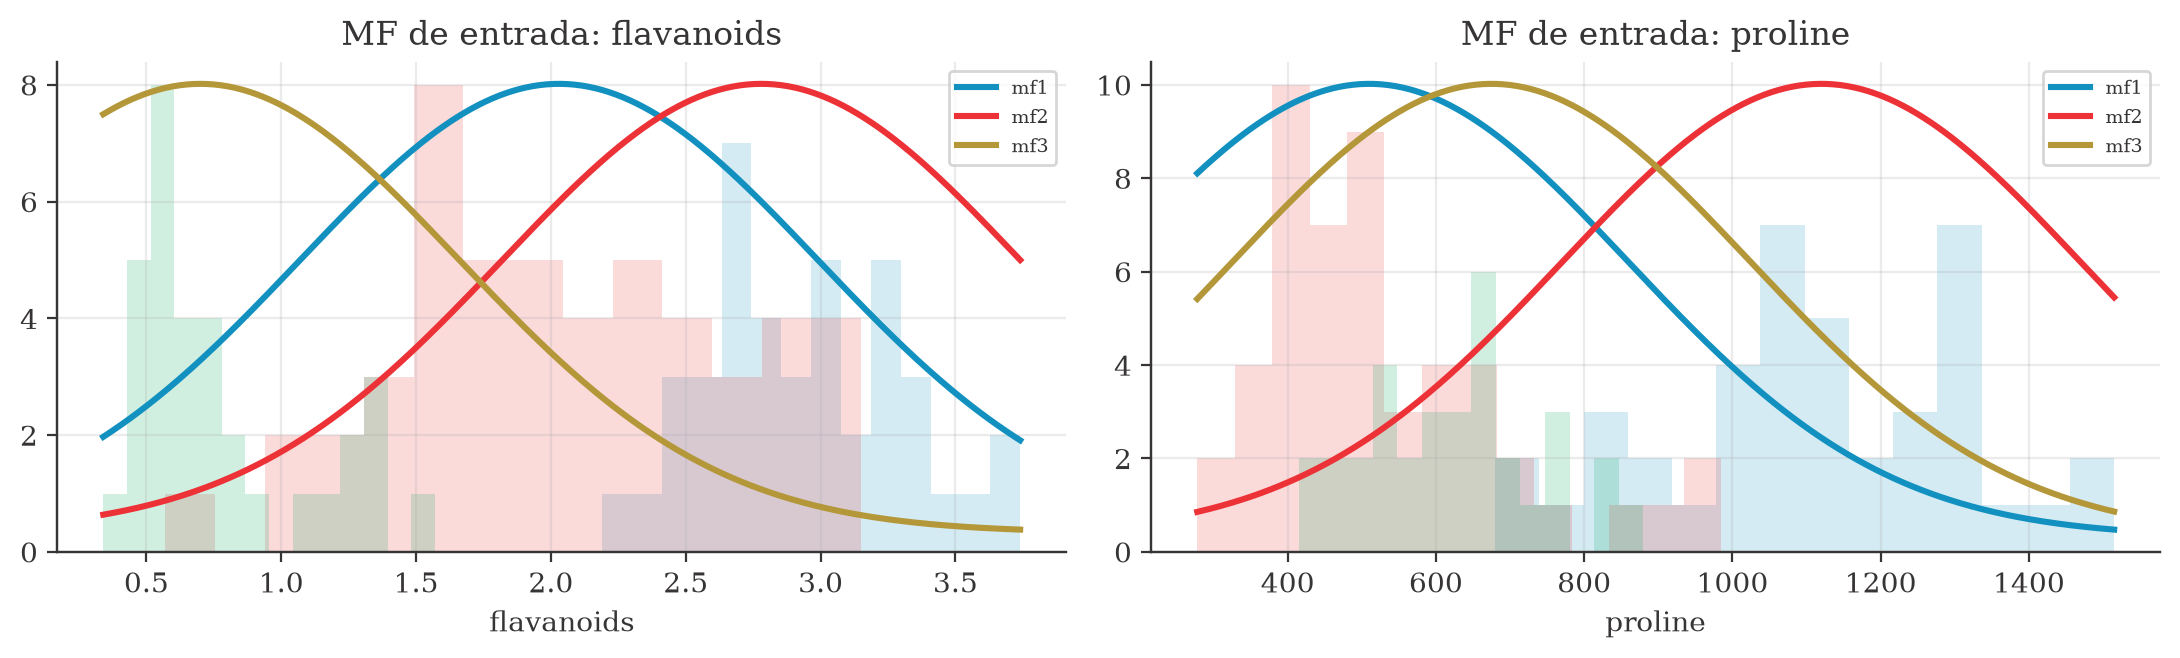
\includegraphics[width=0.88\linewidth]{figuras/prop_f04_mf_entrada.png}\\[2pt]
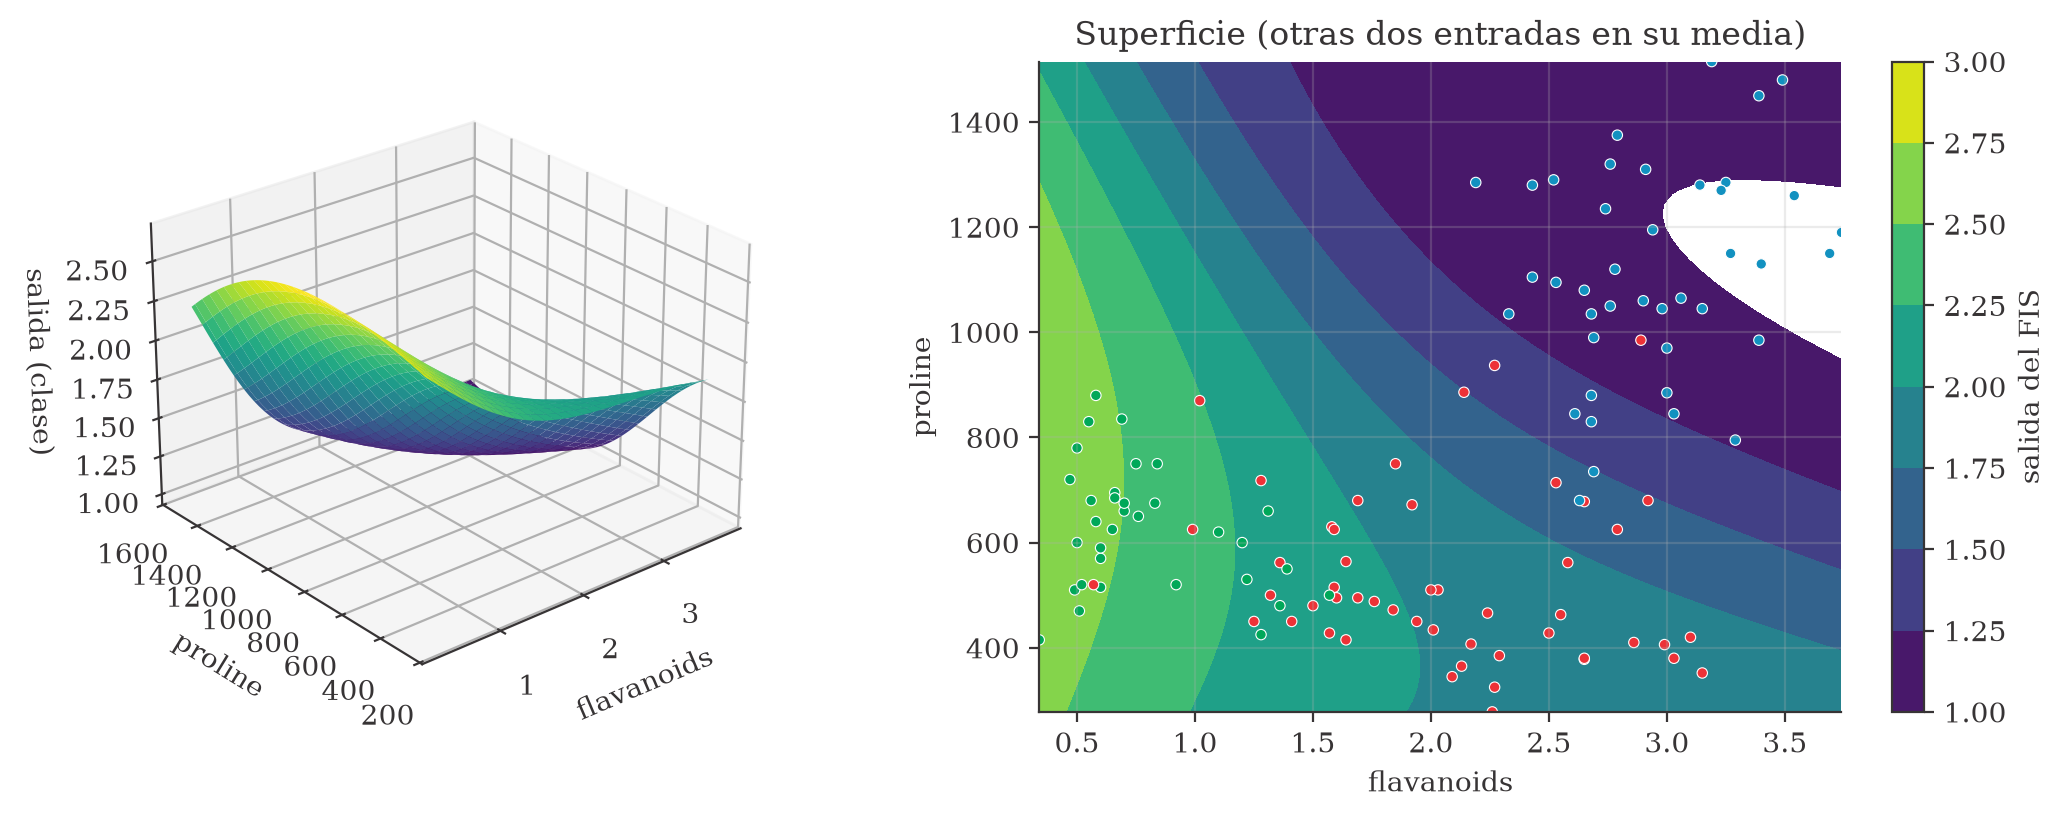
\includegraphics[width=0.72\linewidth]{figuras/prop_f05_superficie.png}
\caption{Vistas de la app: funciones de pertenencia de dos entradas (sobre el histograma por clase) y superficie de flavonoides $\times$ prolina.}
\end{figure}

\begin{table}[H]
\centering\small
\caption{Las 3 reglas de \texttt{fisSub} (centro de cada MF) y la clase que cada una representa.}
\begin{tabular}{lrrrrrrr}
\toprule
Regla & flavanoids & proline & OD280 & alcohol & Vinos & Clase & Pureza \\
\midrule
R1 & 2,03 & 510 & 3,17 & 12,25 & 44 & 2 & 0,98 \\
R2 & 2,78 & 1120 & 3,03 & 13,56 & 42 & 1 & 0,95 \\
R3 & 0,70 & 675 & 1,75 & 12,96 & 38 & 3 & 0,87 \\
\bottomrule
\end{tabular}

\end{table}

\textbf{¿Qué regla es más fácil de leer?} R2 (\textit{flavonoides, prolina, OD280 y alcohol altos $\to$ clase 1}, pureza 0,95): las cuatro condiciones apuntan en el mismo sentido, como anticipaba el ranking de F. R3 (flavonoides y OD280 bajos $\to$ clase 3) también se lee bien.
R1 (clase 2, pureza 0,98) es la más precisa pero se define por contraste (prolina y alcohol bajos). Las gaussianas de cada entrada se traslapan casi por completo: suavizan la superficie pero obligan a nombrar las etiquetas a mano.

\subsection{Extra: ajuste de parámetros (\textit{Tune FIS})}
El enunciado remite al ejemplo de MathWorks (\texttt{openExample("fuzzy/TuneAFuzzyInferenceSystemExample")}), que no se pudo ejecutar. Se adaptó su protocolo: sobre \texttt{fisSub}, entrenado con las filas impares, se ajustan centros y anchos de las MF y se mide el RMSE en las filas pares.

\begin{table}[H]
\centering\small
\caption{Efecto del ajuste sobre el RMSE (en unidades de clase).}
\begin{tabular}{lrr}
\toprule
 & RMSE entrenamiento & RMSE validación \\
\midrule
Antes del ajuste & 0,1452 & 0,2604 \\
Con parada temprana (iteración 1) & 0,0947 & 0,2543 \\
Sin parada (40 iteraciones) & 0,0006 & 0,3840 \\
\bottomrule
\end{tabular}

\end{table}

Sin control el optimizador \textbf{memoriza}: el RMSE de validación sube de \cifratuneValAntes{} a \cifratuneValSin{} (+\cifratuneValSubida\,\%) porque hay 31 parámetros para 62 filas. Con parada temprana (iteración \cifratuneIter) baja a \cifratuneValDesp{} y la exactitud en prueba pasa de
\cifratuneAccAntes{} a \cifratuneAccDesp. Es la lección del Taller 2: sin validación, optimizar más no es mejorar.

\subsection{Extra: 20 particiones y numeración de las clases}\label{sec:veinte}
\begin{table}[H]
\centering\small
\caption{Exactitud en prueba (media $\pm$ desviación) en 20 particiones; la selección de características se rehace en cada una.}\label{tab:veinte}
\begin{tabular}{lrr}
\toprule
Método & Reglas & Exactitud en prueba \\
\midrule
Wang-Mendel n = 2 & 9,7 $\pm$ 1,2 & 0,806 $\pm$ 0,049 \\
Wang-Mendel n = 3 & 24,1 $\pm$ 3,4 & 0,865 $\pm$ 0,047 \\
Wang-Mendel n = 4 & 41,9 $\pm$ 2,9 & 0,931 $\pm$ 0,036 \\
Sustractivo r = 0,3 & 14,8 $\pm$ 2,8 & 0,881 $\pm$ 0,078 \\
Sustractivo r = 0,5 & 5,0 $\pm$ 0,9 & 0,956 $\pm$ 0,024 \\
Sustractivo r = 0,8 & 3,0 $\pm$ 0,0 & 0,946 $\pm$ 0,024 \\
Árbol de 8 hojas & 8 & 0,894 $\pm$ 0,044 \\
\bottomrule
\end{tabular}

\end{table}

El sustractivo con $r=0{,}5$ a $0{,}8$ es el mejor y el más pequeño (3 a 5 reglas frente a unas 42); su diferencia es menor que la desviación y $r=0{,}3$ es el más inestable. Las desviaciones de 0,03 a 0,05 equivalen a 2 o 3 vinos, así que una sola partición no es confiable.
Además, redondear la salida del Sugeno supone clases ordenadas: al permutar las etiquetas (6 numeraciones), el sustractivo logra \cifrapropPermMax{} con la numeración natural o la inversa y baja hasta \cifrapropPermMin{} con las otras cuatro, mientras que
Wang--Mendel no cambia (\cifrapropPermWM). Funciona en \textit{Wine} porque su numeración ya es ordinal.

%% ---------------------------------------------------------------------------------------------
\section{Lectura honesta y reproducibilidad}
\begin{itemize}
  \item \textbf{No se ejecutó MATLAB:} la app \textit{Fuzzy Logic Designer}, \texttt{tunefis} y el ejemplo de MathWorks se reprodujeron en Python (vistas e idea).
  \item \textbf{Prueba pequeña:} con 54 vinos, las diferencias de una partición no son concluyentes; se confirmaron con 20 particiones.
  \item \textbf{Reproducir:} \texttt{make notebooks} (menos de 2 minutos); semilla 42; 29 verificaciones \texttt{[OK]}.
\end{itemize}

\end{document}
